% Artigo do Lab03 (Mineração de métricas DORA) no template SBC.
% Uso no Overleaf: abra o "SBC Conferences Template", substitua o conteúdo do .tex
% principal por este arquivo e envie a pasta figuras/ (4 imagens PNG).
% Trechos em vermelho marcados como [PENDENTE] precisam ser preenchidos pelo grupo.

\documentclass[12pt]{article}

\usepackage{sbc-template}
\usepackage{graphicx,url}
\usepackage[utf8]{inputenc}
\usepackage[T1]{fontenc}
\usepackage[brazil]{babel}
\usepackage{booktabs}
\usepackage{xcolor}
\usepackage{amsmath}
\usepackage[hidelinks]{hyperref}

\newcommand{\pendente}[1]{\textcolor{red}{\textbf{[PENDENTE: #1]}}}

\sloppy

\title{Mineração de Métricas DORA em Repositórios Open-Source:\\
o Quanto Podemos Confiar nos Proxies do GitHub?}

% Confirmar a grafia completa dos nomes antes de enviar.
\author{José Miguel\inst{1}, Eddie Christian\inst{1}, Pedro Talma Toledo\inst{1}}

\address{Curso de Engenharia de Software -- Pontifícia Universidade Católica de Minas
Gerais (PUC Minas)\\ Belo Horizonte -- MG -- Brasil}

\begin{document}

\maketitle

\begin{abstract}
DORA metrics are the de facto standard for measuring software delivery performance,
but GitHub records neither production deployments nor production failures. We mined
the four DORA metrics from 300 popular open-source repositories that use GitHub
Actions, using releases, commits and workflow runs as proxies, and measured how much
the conclusions depend on the operational definitions. The typical repository
publishes one release every three weeks, has a lead time of 8 to 13 days, a CI
failure rate of 5.6\% and recovers from a failing pipeline in 3.7 hours, which places
most repositories in the High and Medium bands. The two failure-rate proxies are
uncorrelated ($\rho = 0.03$), repository age and number of contributors are associated
with slower delivery but not with stability, and changing the operational definition
moves 21\% to 37\% of the repositories to another DORA category.
\end{abstract}

\begin{resumo}
As métricas DORA são o padrão de mercado para medir o desempenho de entrega de
software, mas o GitHub não registra deploys nem falhas em produção. Mineramos as
quatro métricas DORA de 300 repositórios open-source populares que usam GitHub
Actions, usando releases, commits e execuções de workflow como \textit{proxies}, e
medimos o quanto as conclusões dependem das definições operacionais. O repositório
típico publica uma release a cada três semanas, tem lead time de 8 a 13 dias, taxa
de falha de CI de 5,6\% e se recupera de um pipeline quebrado em 3,7 horas, o que
coloca a maioria nas categorias High e Medium. Os dois \textit{proxies} de taxa de
falha não se correlacionam ($\rho = 0{,}03$), a idade e o número de contribuidores se
associam a entregas mais lentas, mas não à estabilidade, e trocar a definição
operacional muda de categoria entre 21\% e 37\% dos repositórios.
\end{resumo}

% =====================================================================
\section{Introdução}

Medir o desempenho de entrega de software exige olhar para duas faces que costumam
ser vistas como opostas: entregar \textbf{rápido} e entregar com \textbf{estabilidade}.
O programa DORA (\textit{DevOps Research and Assessment}), popularizado por
\cite{forsgren2018}, propôs quatro métricas que se tornaram padrão de mercado. A
\textit{frequência de deploy} e o \textit{lead time for changes} medem velocidade; a
\textit{taxa de falha das mudanças} (CFR) e o \textit{tempo de recuperação} medem
estabilidade \cite{dora2024}. Um achado central do DORA é que as duas dimensões não
formam um \textit{trade-off}: as melhores equipes vão bem em ambas.

Essas métricas vêm de questionários respondidos por profissionais. Neste trabalho,
investigamos se elas podem ser \textbf{mineradas} a partir de dados públicos do GitHub.
O problema é que o GitHub não registra deploys nem falhas em produção, e cada métrica
precisa de um \textit{proxy}: uma release publicada é tratada como deploy, e uma
execução de CI com falha, ou uma release corrigida em poucos dias, é tratada como
falha. Por isso, além de descrever o desempenho, avaliamos o quanto as conclusões
dependem dessas escolhas. As questões de pesquisa são:

\begin{itemize}
\item \textbf{RQ01--RQ04.} Quais são a frequência de deploy, o lead time, a taxa de
falha e o tempo de recuperação de repositórios populares que usam CI/CD?
\item \textbf{RQ05.} Repositórios que fazem mais deploys falham mais ou menos?
\item \textbf{RQ06.} Quais características dos repositórios se associam a um melhor
desempenho DORA?
\item \textbf{RQ07.} O quanto a classificação DORA depende da definição operacional?
\end{itemize}

Antes da coleta, registramos hipóteses informais. \textbf{H1}: mediana de 0,25 a 0,75
release por semana (Medium), com cauda longa e poucos repositórios Low. \textbf{H2}:
lead time de 2 a 4 semanas por release e de cerca de 1 semana por commit.
\textbf{H3}: CFR de CI entre 10\% e 25\%, CFR de entrega entre 10\% e 20\% e
correlação fraca entre os dois. \textbf{H4}: recuperação mediana de 1 a 12 horas,
com cauda longa e recuperação mais lenta em projetos com menos contribuidores.
\textbf{H5}: associação fraca entre frequência e CFR de CI e positiva com o CFR de
entrega. \textbf{H6}: mais contribuidores se associam a entregas mais rápidas, e a
popularidade não se associa ao desempenho. \textbf{H7}: ao menos 20\% dos
repositórios mudam de categoria ao trocar a definição, com kappa abaixo de 0,80.

% =====================================================================
\section{Metodologia}

\subsection{Fonte de dados, janela e funil de seleção}

Os dados vêm da API REST do GitHub, coletados por um pipeline próprio em Python, sem
bibliotecas prontas de acesso à API. O pipeline guarda cada resposta em cache local,
o que permite retomar uma coleta interrompida, espera automaticamente quando a cota
da API acaba e repete com espera crescente as requisições que falham por erro do
servidor. A coleta roda com um único comando, e os parâmetros ficam num arquivo de
configuração. A \textbf{janela de observação} vai de 1º de outubro de 2025 a 30 de
setembro de 2026 (UTC); só entram releases e execuções de CI desse período.

Buscamos repositórios com pelo menos 1.000 estrelas, não arquivados e com algum
\textit{push} na janela. Como a busca devolve no máximo 1.000 resultados por
consulta, ela é dividida em faixas de estrelas, e cada faixa que passa do limite é
dividida ao meio automaticamente. Os candidatos são embaralhados com semente fixa e
avaliados em ordem até a amostra atingir 300 repositórios. Cada um é descartado no
primeiro filtro em que falhar: (1)~usar GitHub Actions; (2)~ter ao menos 5 releases
publicadas na janela, sem rascunhos nem pré-releases; e (3)~ter ao menos 50 execuções
de CI válidas no \textit{default branch}, disparadas por \texttt{push} e concluídas
com sucesso ou falha. A Tabela~\ref{tab:funil} mostra o funil. O filtro de releases é
o mais restritivo: 65\% dos repositórios com Actions não publicaram 5 releases na
janela.

\begin{table}[ht]
\centering
\caption{Funil de seleção dos repositórios.}\label{tab:funil}
\small
\begin{tabular}{lrr}
\toprule
Etapa & Restantes & Descartados \\
\midrule
Candidatos da busca & 37.611 & -- \\
Avaliados até completar a amostra & 1.447 & 36.164 \\
Com GitHub Actions & 1.177 & 270 \\
Com $\geq$ 5 releases na janela & 407 & 770 \\
Com $\geq$ 50 execuções de CI válidas & \textbf{300} & 107 \\
\bottomrule
\end{tabular}
\end{table}

\subsection{Definições operacionais e variantes}

\textbf{Frequência de deploy:} releases estáveis publicadas na janela divididas pelo
número de semanas (52,1). \textbf{Lead time:} para cada release, obtemos os commits
incluídos comparando-a com a release estável anterior, que pode estar fora da janela;
a data de um commit é \texttt{commit.author.date}. Na variante (a), o lead time da
release é o tempo desde o commit mais antigo até a publicação, e o valor do
repositório é a mediana entre releases. Na variante (b), cada commit contribui com o
seu próprio tempo, e a mediana é tomada sobre todos os commits. A primeira release da
história e comparações indisponíveis (por exemplo, erro 404) não recebem lead time.
\textbf{CFR (a), proxy de CI:} execuções com conclusão \texttt{failure},
\texttt{timed\_out} ou \texttt{startup\_failure} divididas pelo total de falhas e
sucessos; execuções canceladas ou puladas são ignoradas. \textbf{CFR (b), proxy de
entrega:} uma release falha quando é seguida, em até 7 dias, por uma release
corretiva, definida por uma heurística que exige mudança só no número de
\textit{patch} da versão SemVer e as palavras \texttt{fix}, \texttt{hotfix} ou
\texttt{revert} nos commits; releases dos últimos 7 dias da janela ficam fora do
denominador (censura). \textbf{Tempo de recuperação:} em cada workflow, um episódio
começa na primeira falha após um sucesso e termina no fim da execução bem-sucedida
seguinte; o valor do repositório é a mediana dos episódios, e episódios não
resolvidos até o fim da janela são contados como censurados.

Cada repositório é classificado em Elite, High, Medium ou Low em cada métrica, com os
cortes fixos da disciplina adaptados dos relatórios DORA. A categoria geral é a
mediana dos pontos (Elite = 4 \ldots{} Low = 1), arredondada para baixo. A
\textbf{combinação de referência C1} usa release, lead time (a) e CFR (a). Para a
RQ07, definimos também \textbf{C2} (release ou pré-release, lead time (b) e CFR (b))
e \textbf{C3} (tag, lead time (b) e CFR (a)); o tempo de recuperação é o mesmo nas três.

\subsection{Validação manual (amostra-ouro)}

Para medir o erro dos critérios automáticos, construímos uma amostra-ouro de
60 repositórios sorteados da amostra final com semente fixa, com 5 releases sorteadas
de cada um. Os avaliadores rotularam, de forma independente e sem ver a saída da
heurística, (i)~o tipo do projeto, (ii)~se as releases representam entregas reais ao
usuário e (iii)~se cada release é corretiva, a partir de uma planilha gerada
automaticamente com links para as releases e os commits. A concordância foi medida
pelo kappa de Fleiss, interpretado pela escala de \cite{landis1977}; o rótulo de
consenso é a maioria simples, e os empates foram decididos em reunião. A heurística
do CFR (b) foi avaliada contra o consenso por precisão, recall e F1, com meta de
F1~$\geq$~0,70. \pendente{refazer o sorteio sobre os 300 finais, concluir a
rotulagem e inserir aqui o kappa de cada dimensão, o número de empates e o F1 de cada
versão da heurística. Registrar que a Pessoa B, de atestado, não participou da
rotulagem, se for o caso.}

% =====================================================================
\section{Resultados}

\subsection{RQ01 a RQ04: métricas DORA}

Como as distribuições são muito assimétricas, reportamos mediana e intervalo
interquartil (IQR). A Tabela~\ref{tab:descritiva} resume as métricas, e a
Figura~\ref{fig:hist} mostra as distribuições com os cortes das categorias.

\begin{table}[ht]
\centering
\caption{Estatística descritiva das métricas (n = repositórios com a métrica).}
\label{tab:descritiva}
\small
\begin{tabular}{llrrrr}
\toprule
RQ & Métrica & n & Mediana & Q1 & Q3 \\
\midrule
RQ01 & Frequência de deploy (releases/semana) & 300 & 0,32 & 0,15 & 0,82 \\
RQ02 & Lead time (a) por release & 300 & 12,8 dias & 3,0 dias & 39,9 dias \\
RQ02 & Lead time (b) por commit & 300 & 8,5 dias & 2,1 dias & 36,5 dias \\
RQ03 & CFR (a) proxy de CI & 300 & 5,6\% & 1,9\% & 14,5\% \\
RQ03 & CFR (b) proxy de entrega & 299 & 11,1\% & 0,0\% & 27,5\% \\
RQ04 & Tempo de recuperação & 279 & 3,7 h & 0,9 h & 20,1 h \\
\bottomrule
\end{tabular}
\end{table}

\begin{figure}[ht]
\centering
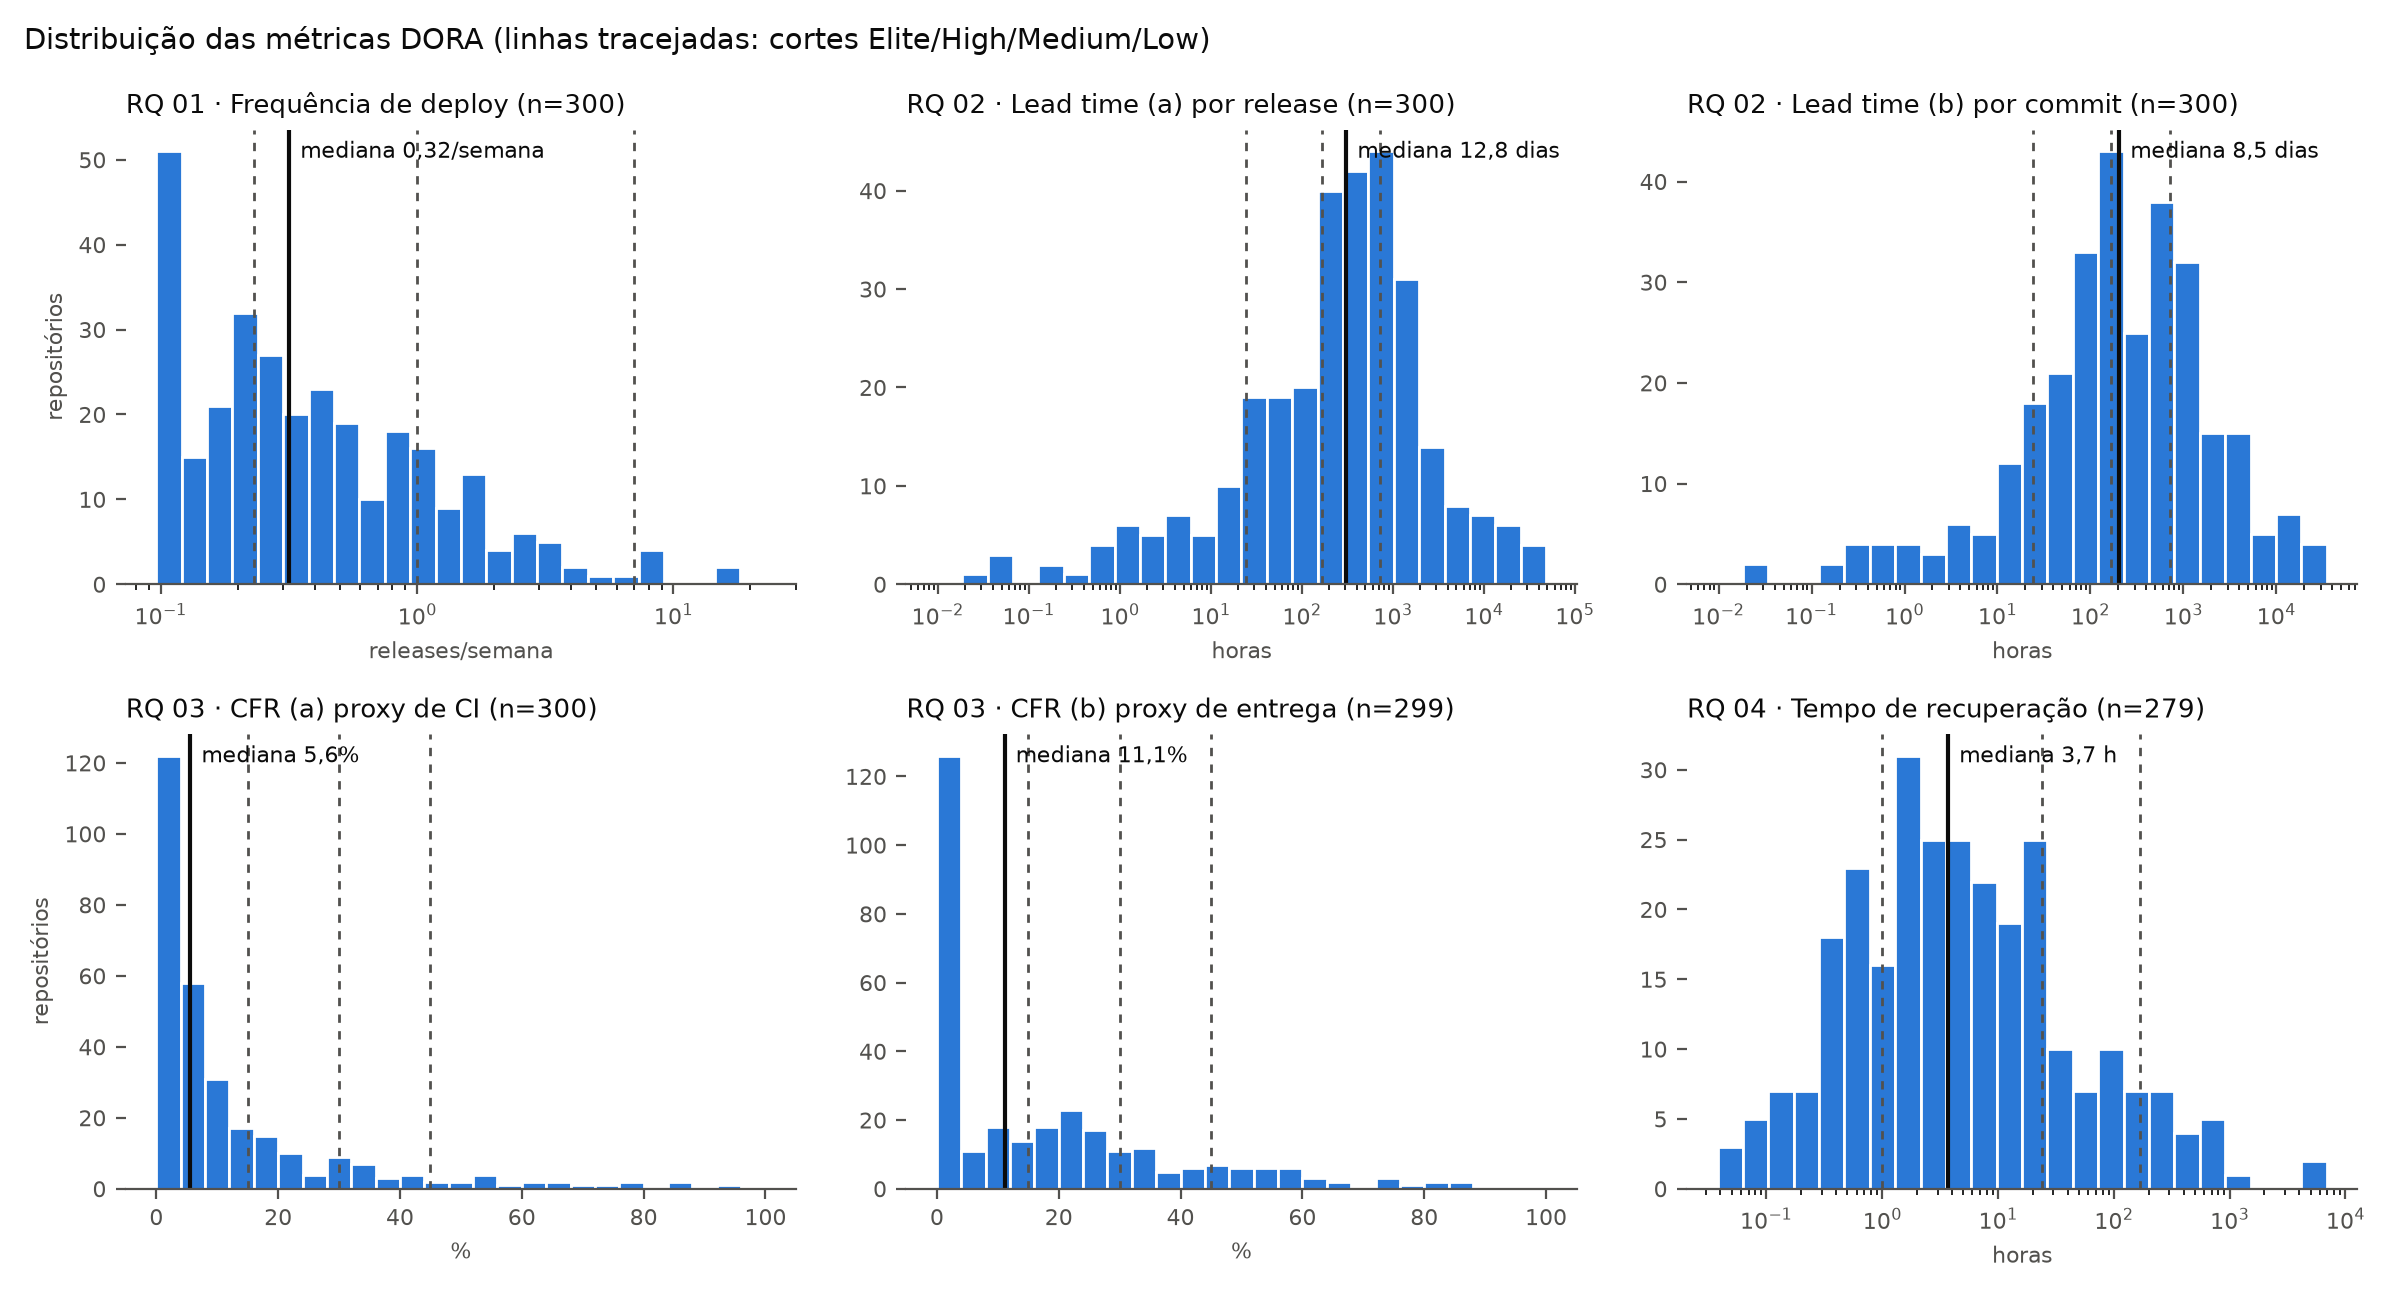
\includegraphics[width=0.92\textwidth]{figuras/rq01_04_histogramas.png}
\caption{Distribuição das métricas. Linhas tracejadas: cortes entre categorias DORA;
linha contínua: mediana. Frequência, lead time e recuperação em escala log.}
\label{fig:hist}
\end{figure}

\textbf{RQ01.} O repositório típico publica 0,32 release por semana, cerca de uma a
cada três semanas. A cauda à direita é longa: 19\% publicam uma ou mais releases por
semana, mas 37\% publicam menos de uma por mês. \textbf{RQ02.} O lead time mediano é
de 12,8 dias por release e 8,5 dias por commit. As variantes são fortemente
correlacionadas ($\rho = 0{,}73$), mas a (a) é maior em 66\% dos repositórios,
porque mede o commit mais antigo de cada release, enquanto a (b) dá o mesmo peso a
todos os commits. \textbf{RQ03.} O CFR de CI tem mediana de 5,6\%, e o de entrega,
11,1\%; 40\% dos repositórios não tiveram nenhuma release marcada como falha. As duas
variantes \textbf{praticamente não se correlacionam} ($\rho = 0{,}03$; $p = 0{,}56$).
\textbf{RQ04.} Um workflow quebrado volta a passar, na mediana, em 3,7 horas. Dos
12.251 episódios de falha, 200 (1,6\%) foram censurados, e 21 repositórios não
tiveram nenhum episódio resolvido.

\textbf{Classificação de referência (C1).} A classificação geral se concentra nas
categorias intermediárias: Medium (43\%) e High (37\%), com 7\% Elite e 13\% Low
(Figura~\ref{fig:categorias}). O CFR (a) é a métrica mais ``generosa'' (76\% Elite),
e a frequência é a mais restritiva (2\% Elite).

\begin{figure}[ht]
\centering
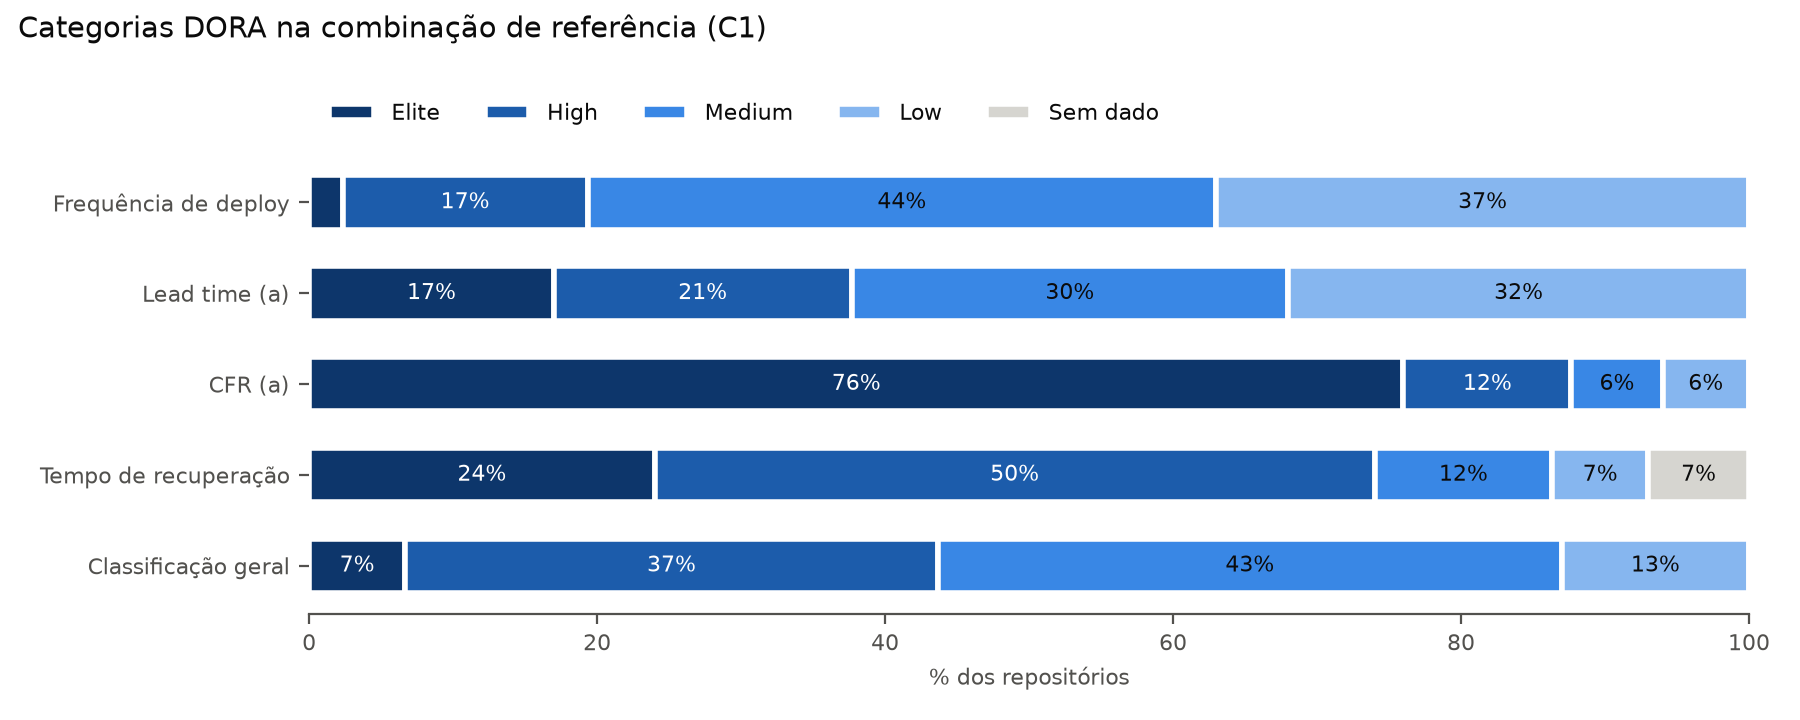
\includegraphics[width=0.9\textwidth]{figuras/rq01_04_categorias_c1.png}
\caption{Categorias DORA por métrica e na classificação geral (C1).}
\label{fig:categorias}
\end{figure}

\subsection{RQ05: frequência de deploy $\times$ taxa de falha}

A correlação de Spearman entre a frequência e o CFR de CI é desprezível
($\rho = 0{,}03$; $p = 0{,}57$; $n = 300$). Com o CFR de entrega, é moderada e
positiva ($\rho = 0{,}35$; $p < 0{,}001$; $n = 299$), como mostra a
Figura~\ref{fig:rq05}.

\begin{figure}[ht]
\centering
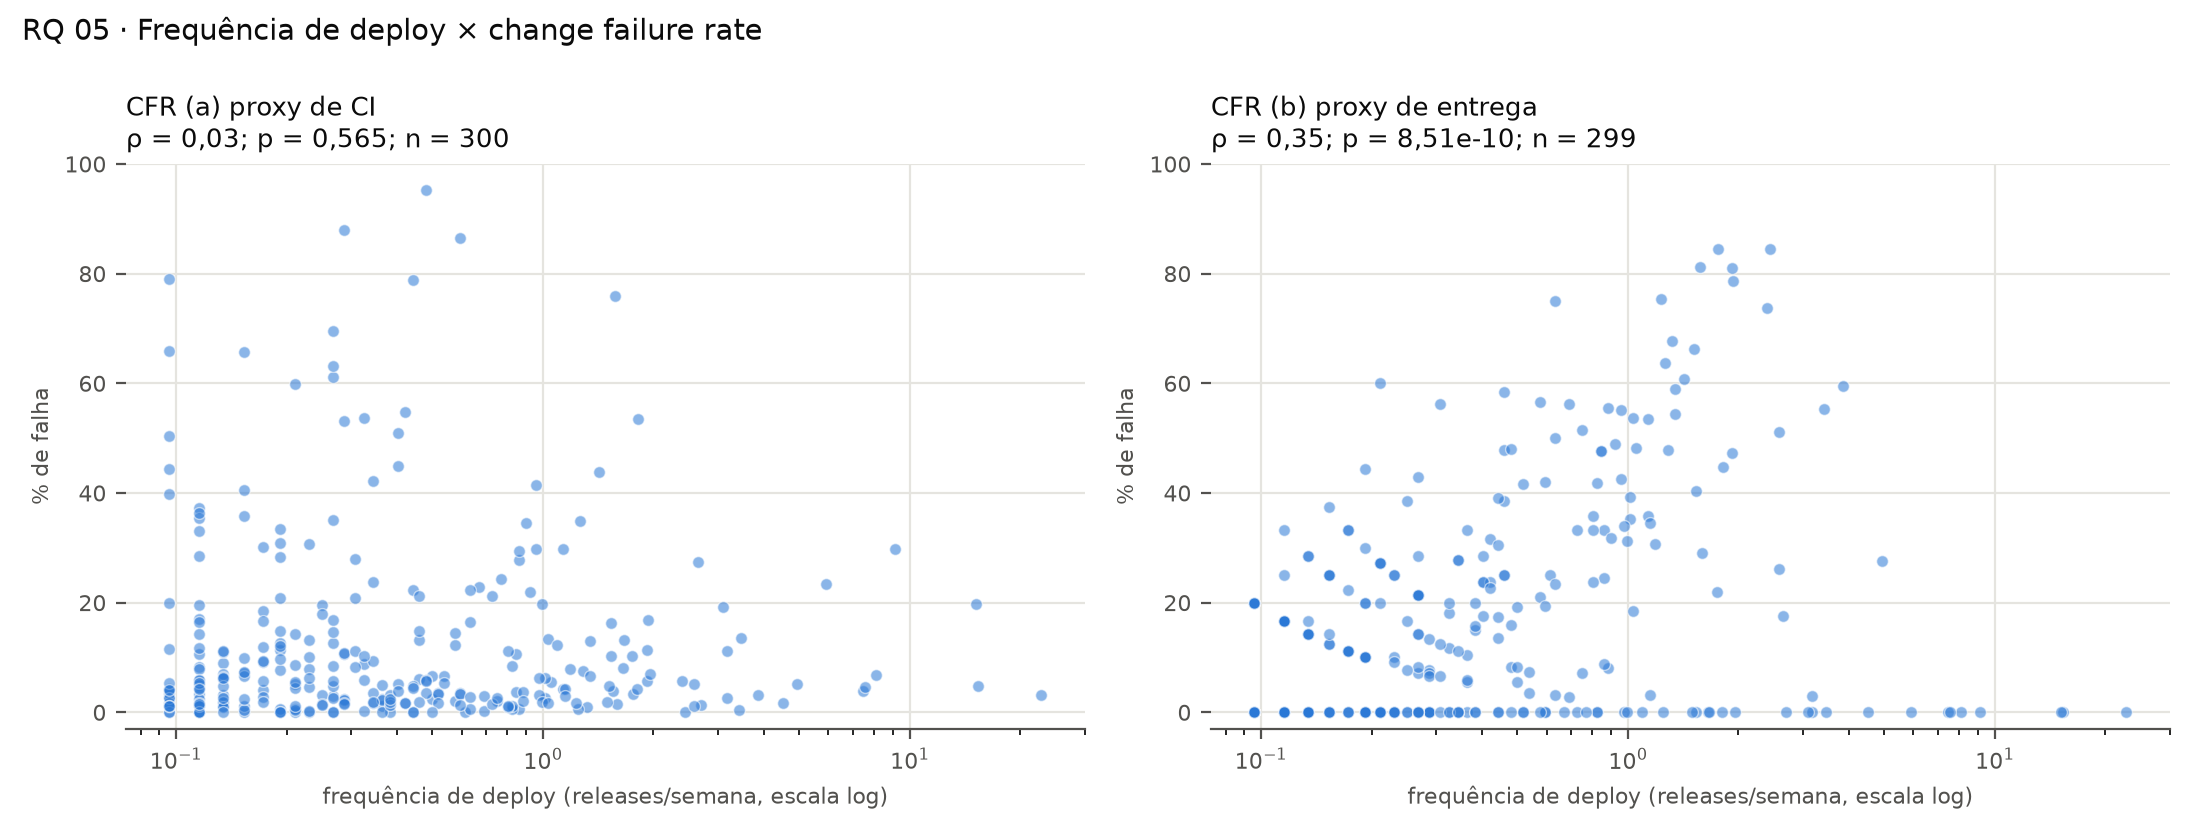
\includegraphics[width=0.85\textwidth]{figuras/rq05_dispersao.png}
\caption{Frequência de deploy (escala log) contra cada variante do CFR.}
\label{fig:rq05}
\end{figure}

\subsection{RQ06: características dos repositórios}

Comparamos as quatro métricas de C1 entre grupos de quatro fatores: estrelas,
contribuidores e idade (em quartis) e linguagem principal (seis linguagens com pelo
menos 15 repositórios e um grupo ``Outras''). Aplicamos Kruskal-Wallis nos 16 pares,
com correção de Holm, e reportamos o tamanho de efeito $\varepsilon^2 = H/(n-1)$,
interpretado por analogia ao $\eta^2$ \cite{cohen1988}, e o Cliff's delta entre o 4º
e o 1º quartil, interpretado por \cite{romano2006}. Quatro associações continuam
significativas após a correção (Tabela~\ref{tab:rq06}, Figura~\ref{fig:rq06}),
\textbf{todas em métricas de velocidade}. Nenhum fator se associou ao CFR (a) ou à
recuperação ($\varepsilon^2 \leq 0{,}034$), e as estrelas não se associaram a nenhuma
métrica.

\begin{table}[ht]
\centering
\caption{Associações significativas após a correção de Holm ($p < 0{,}001$ em todas).}
\label{tab:rq06}
\small
\begin{tabular}{llrlr}
\toprule
Fator & Métrica & $\varepsilon^2$ & Medianas por grupo & $\delta$ (Q4$\times$Q1) \\
\midrule
Idade & Lead time (a) & 0,23 & Q1 2,5 dias $\rightarrow$ Q4 38,3 dias & 0,69 \\
Contribuidores & Lead time (a) & 0,15 & Q1 3,2 dias $\rightarrow$ Q4 30,0 dias & 0,61 \\
Idade & Frequência & 0,15 & Q1 0,84 $\rightarrow$ Q4 0,19 por semana & $-$0,57 \\
Linguagem & Lead time (a) & 0,11 & TypeScript 5,1 dias; C++ 37,1 dias & -- \\
\bottomrule
\end{tabular}
\end{table}

\begin{figure}[ht]
\centering
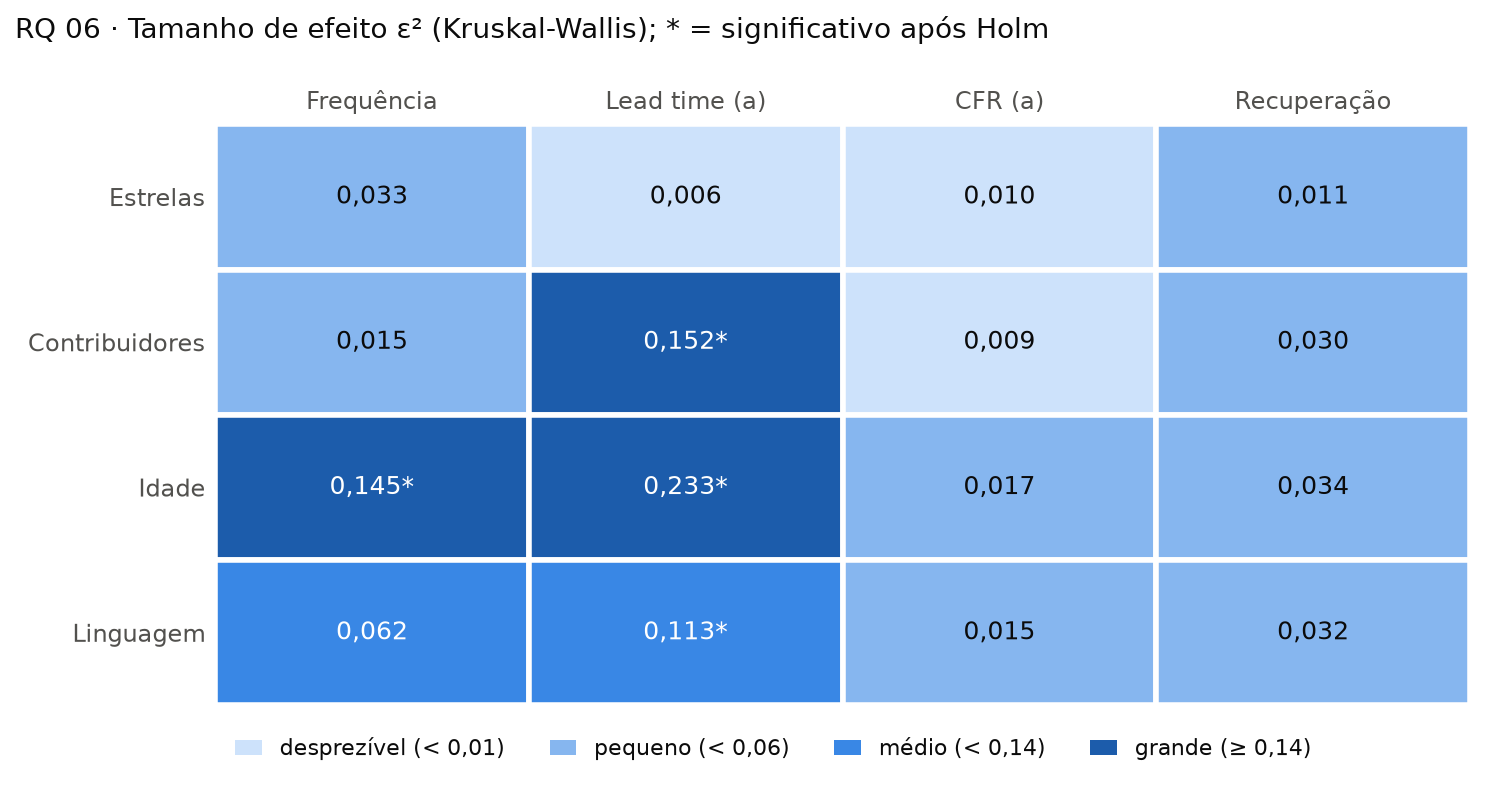
\includegraphics[width=0.72\textwidth]{figuras/rq06_efeitos.png}
\caption{$\varepsilon^2$ de cada teste; * indica $p < 0{,}05$ após Holm.}
\label{fig:rq06}
\end{figure}

\subsection{RQ07: sensibilidade à definição operacional}

Classificamos cada repositório nas combinações C1, C2 e C3 e comparamos os pares que
têm as quatro métricas nos dois cenários (Tabela~\ref{tab:rq07}). Entre um quinto e
mais de um terço dos repositórios mudam de categoria. O par C1$\times$C2 é o menos
estável, e a maior parte das mudanças vem da taxa de falha: a categoria do CFR muda em
157 dos 300 repositórios entre C1 e C2. Em C3, a frequência medida por tags é maior
(mediana de 0,44 contra 0,32 por semana) e os repositórios tendem a subir de
categoria. Quase todas as mudanças são de um único nível.

\begin{table}[ht]
\centering
\caption{Mudança de categoria geral entre combinações (kappa de Cohen ponderado linear).}
\label{tab:rq07}
\small
\begin{tabular}{lrrrrr}
\toprule
Par & n & Mudaram & Subiram & Desceram & $\kappa$ \\
\midrule
C1 $\times$ C2 & 278 & 102 (36,7\%) & 49 & 53 & 0,47 \\
C1 $\times$ C3 & 279 & 58 (20,8\%) & 43 & 15 & 0,74 \\
C2 $\times$ C3 & 278 & 69 (24,8\%) & 50 & 19 & 0,64 \\
\bottomrule
\end{tabular}
\end{table}

% =====================================================================
\section{Discussão}

\textbf{H1 foi confirmada em parte.} A mediana caiu na faixa prevista, mas 37\% dos
repositórios ficaram em Low: o piso do filtro (cerca de 0,1 release por semana) está
bem abaixo do corte de Low (0,23), então um projeto com 5 a 11 releases por ano entra
na amostra e é classificado como Low. \textbf{H2 foi confirmada}, com valores um pouco
menores que o previsto para a variante (a), provavelmente porque \textit{patches}
publicados poucos dias após uma versão maior puxam a mediana para baixo.
\textbf{H3 foi confirmada em parte.} O CFR de entrega ficou na faixa prevista, mas o
de CI ficou abaixo (5,6\%), provavelmente porque o código já passou pela CI do
\textit{pull request} antes de chegar ao \textit{default branch}. A ausência de
correlação entre as variantes mostra que falha de pipeline e falha percebida pelo
usuário são fenômenos distintos. \textbf{H4 foi confirmada} quanto ao valor típico e
à cauda longa, mas a censura foi menor que o esperado, e a relação com o número de
contribuidores não se sustentou após a correção para comparações múltiplas.

\textbf{H5 foi confirmada}, mas os dados \textbf{não sustentam um trade-off} entre
velocidade e estabilidade. Pelo proxy de CI, as duas dimensões são independentes. A
correlação positiva com o CFR de entrega decorre em boa parte da própria definição:
releases corretivas também contam como deploys, e quem publica mais tem mais pares de
releases separados por menos de 7 dias. Também não reproduzimos a afirmação do DORA
de que os mais rápidos são os mais estáveis. \textbf{H6 foi refutada para os
contribuidores}: projetos com mais contribuidores, e principalmente os mais antigos,
entregam \textit{mais devagar}. As duas variáveis são correlacionadas ($\rho = 0{,}53$),
e uma explicação plausível é que projetos maduros adotam ciclos de release mais longos
e planejados. Como previsto, a popularidade não se associou ao desempenho, e nenhum
fator explicou a estabilidade, que parece depender mais de práticas de cada projeto.

\textbf{H7 foi confirmada.} Os resultados agregados são robustos: em todas as
combinações, a maioria dos repositórios fica em High ou Medium. Já a classificação de
um repositório específico não é robusta, porque depende principalmente do proxy de
falha escolhido. Comparar projetos individuais por métricas DORA mineradas do GitHub
exige declarar as definições operacionais e, de preferência, mostrar mais de uma.

% =====================================================================
\section{Ameaças à validade}

Seguimos as categorias de \cite{wohlin2012}.

\textbf{Construto.} Nenhuma métrica observa diretamente o fenômeno do DORA. Release
não é deploy: para bibliotecas, quem coloca a versão em produção são os usuários, e
aplicações podem fazer deploy contínuo sem releases. Falha de CI não é falha em
produção: o pipeline barra justamente as falhas que detecta, e a correlação quase nula
entre os dois CFRs é evidência disso. A heurística de release corretiva pode errar, e
\texttt{commit.author.date} é afetada por \textit{rebases} e \textit{squash merges}.
Em projetos que mantêm várias linhas de versão em paralelo, a release anterior por
data pode pertencer a outra linha e inflar o lead time.

\textbf{Interna.} Fatores não medidos podem explicar as associações da RQ06, como o
tipo do projeto e a correlação entre idade e contribuidores. Repositórios com CI
disparada por bots distorcem o CFR (a) e a recuperação; um deles teve a coleta de CI
incompleta. Releases e tags apagadas ou reescritas alteram o histórico observado.

\textbf{Externa.} A amostra tem apenas projetos populares, com GitHub Actions e que
publicam releases; o filtro de releases excluiu 65\% dos repositórios com Actions. Os
resultados não valem para equipes corporativas, base dos relatórios DORA, nem para
outras janelas de tempo, e as linguagens menos frequentes estão sub-representadas.

\textbf{Conclusão.} A RQ06 fez 16 testes; aplicamos a correção de Holm, e quatro
resultados com $p < 0{,}05$ sem correção deixaram de ser significativos. Reportamos
tamanhos de efeito porque, com $n = 300$, até diferenças pequenas podem ser
significativas. Alguns grupos de linguagem são pequenos (18 repositórios em C++), e os
fatores, testados separadamente, são correlacionados entre si.

% =====================================================================
\section{Replicação cruzada}

\pendente{relatar a execução do pipeline do grupo sorteado usando apenas o README
(30 repositórios), a diferença relativa por métrica, a porcentagem de repositórios com
a mesma classificação DORA, as Issues abertas e as Issues recebidas e respondidas.}

% =====================================================================
\section{Conclusão}

Mineramos as quatro métricas DORA de 300 repositórios open-source populares. O
repositório típico tem desempenho intermediário: entrega a cada poucas semanas, com
lead time de uma a duas semanas, CI estável e recuperação em poucas horas. Velocidade
e estabilidade não mostraram \textit{trade-off}, e as características dos projetos se
associam só à velocidade. A principal lição, porém, é metodológica: os
\textit{proxies} de falha medem fenômenos diferentes, e a escolha da definição
operacional muda a categoria de até um terço dos repositórios. Métricas DORA mineradas
do GitHub são úteis para descrever populações de projetos, mas devem ser usadas com
cautela para avaliar projetos individuais.

\textbf{Disponibilidade.} Código, dados e análises:
\url{https://github.com/JoseMiguel-ofc/LABORATORIO-DE-EXPERIMENTACAO-DE-SOFTWARE}
(pasta \texttt{LABORATORIO 03}). GitHub Projects: \pendente{colar o link do quadro do
GitHub Projects}.

% =====================================================================
\begin{thebibliography}{9}

\bibitem[Cohen 1988]{cohen1988}
Cohen, J. (1988).
\newblock {\em Statistical Power Analysis for the Behavioral Sciences}.
\newblock Lawrence Erlbaum, 2nd edition.

\bibitem[DORA 2024]{dora2024}
DORA (2024).
\newblock DORA's software delivery metrics: the four keys.
\newblock \url{https://dora.dev/guides/dora-metrics-four-keys/}.

\bibitem[Forsgren et~al. 2018]{forsgren2018}
Forsgren, N., Humble, J., and Kim, G. (2018).
\newblock {\em Accelerate: The Science of Lean Software and DevOps}.
\newblock IT Revolution.

\bibitem[Landis and Koch 1977]{landis1977}
Landis, J.~R. and Koch, G.~G. (1977).
\newblock The measurement of observer agreement for categorical data.
\newblock {\em Biometrics}, 33(1):159--174.

\bibitem[Romano et~al. 2006]{romano2006}
Romano, J., Kromrey, J.~D., Coraggio, J., and Skowronek, J. (2006).
\newblock Appropriate statistics for ordinal level data.
\newblock In {\em Annual Meeting of the Florida Association of Institutional Research}.

\bibitem[Wohlin et~al. 2012]{wohlin2012}
Wohlin, C., Runeson, P., Höst, M., Ohlsson, M.~C., Regnell, B., and Wesslén, A. (2012).
\newblock {\em Experimentation in Software Engineering}.
\newblock Springer.

\end{thebibliography}

\end{document}
